\documentclass{article}
%\usepackage{ctex}
\usepackage[fntef]{ctexcap}
\setCJKmainfont{楷体}
\CTEXsetup[number={\chinese{section}},format={\Large\bfseries}]{section}

\begin{document}
	\author{北京邮电大学 机器人队}
	\tableofcontents
	\pagebreak
\section{前言}
\subsection{本文适用人群}

\begin{enumerate}
	\item 不满足于上层软件设计,想弄清硬件运行原理的DIY爱好者
	\item 对电子技术、软件编程感兴趣而不知从何入手
	\item 有意向参加机器人、智能车等软硬综合比赛
	\item 机器人爱好者、模型(航模、车模)爱好者
\end{enumerate}
本文主要面向北京邮电大学大一、大二学生,作为北邮机器人队预备队的教程,当然也欢迎其他爱好者参考。

\subsection{本文主要内容}
\begin{enumerate}
	\item 飞行器相关介绍
	\item 常见电子执行器件(电机、舵机)及其驱动方式介绍
	\item PCB设计(原理图设计及Layout)
	\item 使用STM32QubeMX根据分配的引脚功能生成工程
	\item 单片机编程
\end{enumerate}

需要注意的是,有些内容与我们整个训练关系不大,会简略跳过,有兴趣的同学请自行对相关关键词进行搜索。同时,软件的安装等也无法很详尽地说明,如果大家对有些软件的安装有所疑问,请配合搜索引擎。

\section{预备知识}
\subsection{无人机、航模}
除了军用无人机,生活中我们所提及的无人机及航模的概念实际上非常接近。目前也没有明确的概念来区分二者,因此本文中不区分这两者概念,统一称为“飞行器”。
\subsection{固定翼飞行器}
固定翼飞行器是生活中最常见的飞行器。常见的客机、战斗机等,都可以归于固定翼飞行器的范畴。与多轴飞行器相比,固定翼飞行器巡航速度快,负载大。
\subsection{如何控制固定翼飞行器?}
固定翼飞行器一般包含主翼、尾翼、机身、发动机等。飞行器的动力来源来自于发动机,对于电动飞行器而言,发动机就是电机。飞行器的拐弯通过主翼上的副翼、及垂直尾翼上的方向舵来控制。爬升则通过水平尾翼上的升降舵来控制。

\begin{figure}[ht]
\centering
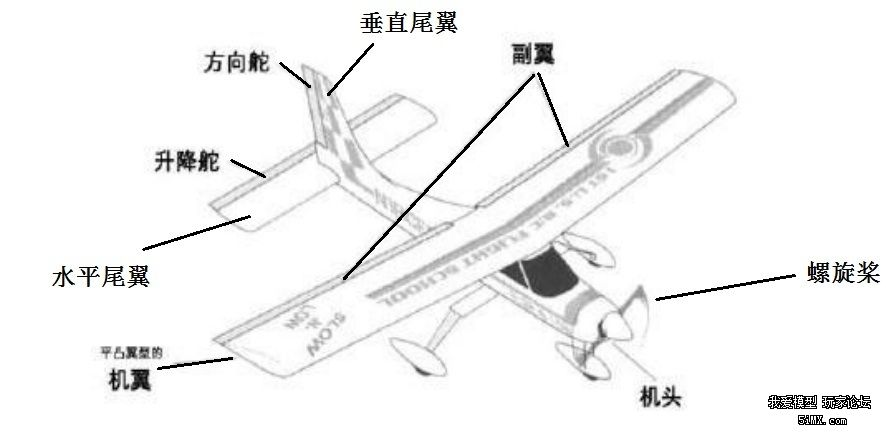
\includegraphics[scale=0.4]{固定翼.jpg}
\caption{固定翼飞机}
\label{fig:label}
\end{figure}


依据伯努利定律,飞行器的升力来自于机翼上下两侧的压力差,因此通过控制左右副翼的升降,可以控制飞行器的“横滚”、控制升降舵的升降,则可以控制飞行器的“俯仰”。

\subsection{控制通道}
常见“三通”、“四通”都指的是飞行器的控制通道。三通一般为三个控制通道:油门、方向舵、升降舵。四通则为油门、方向舵、副翼、升降舵。当然了,也可以自制无动力的三通滑翔机,则此时三个通道为:副翼、方向舵、升降舵。

\subsection{执行器件及其控制方式}
电机,飞行器上常用直流电机,包括空心杯电机及无刷电机。在飞行器上一般使用空心杯电机。
空心杯电机是一种常见的有刷电机,想必大家小时候都玩过四驱车,里面的马达就是一种有刷电机。在中学物理中,大家学的电动机模型就是有刷电机。控制有刷电机的方式很简单,通过在电机两端加上一定的电压,即可驱动有刷电机,而改变电压的大小,即可调速。
\begin{figure}[ht]
\centering
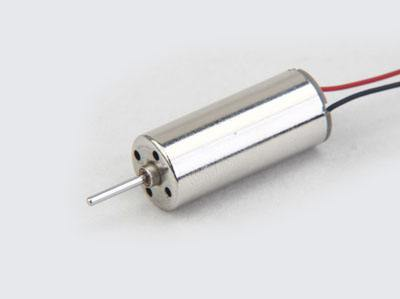
\includegraphics[scale=0.4]{空心杯.jpg}
\caption{空心杯电机}
\label{fig:label}
\end{figure}

无刷电机,是航模的主要动力,动力强劲,重量也比一般的有刷电机(除了空心杯)轻很多。无刷电机的驱动较为复杂,因为无刷电机内部没有一种叫做“电刷”的东西,因此得通过外部进行电流的换向。驱动无刷电机不能直接在两端施加电压,而应外接一个叫做“电子调速器”的东西,俗称电调。通过改变输给电调信号的“脉宽”(即高电平宽度),来实现无刷电机的调速。

舵机,是航模上控制舵面( 升降舵、副翼、方向舵)的主要元件。舵机内部包含了简单的控制电路,对舵机输入一定的“脉宽”,即可使舵机转动到相应位置。

\section{材料清单}
下面列出制作一个微型固定翼飞行器所需要的清单,出于训练的目的,飞行器的电路板及程序都由我们自己设计及编写。

1、Jbug空机

2、720空心杯电机*2

3、电磁舵机或微型舵机*2

4、电路板

5、1S 锂电池

\section{控制器选型}
我们的目标是设计一个可以控制(通过电脑或者手机)的飞行器,而且程序的编写尽量的简洁,不涉及太多单片机底层的操作。(实际上,等你接触过许多单片机,你会发现在单片机底层上浪费的时间是很不值得的)

因此我们选择了ST的一个常见型号,STM32F103C8T。32位单片机,72M主频,对我们的需求绰绰有余。更主要的是,ST的官方工具STM32QubeMX非常好用,能让我们将更多精力聚焦于控制与算法,而不是配置IO口功能。

\section{控制电路设计}
\subsection{AD软件简介}
Alitum Designer是一个简单的PCB设计软件。设计PCB的一般流程是通过在原理图定义各个网络名及其连接,接着在PCB文件中通过走线将各个元件实际上连接起来。
该软件可以在BT上下载。

\subsection{单片机最小系统设计}
所谓单片机的最小系统,即指能使单片机运行起来的最小单元,一般包含给单片供电的电源电路、程序下载及调试电路、晶振电路、复位电路,及相应的LED提示电路等。

需要注意的是,这里设计了一些接在3.3V与GND之间的电容,目的就是对电源进行滤波,以防止电源波动较大,对程序运行产生影响。这些电容也叫做去耦电容。

\subsection{电机驱动电路设计}
因为本飞行器使用的是空心杯电机,前面提到,控制空心杯的方式非常简单,只要改变电压即可调速。而在电路上设计一个可控的电压源是比较麻烦的是,因此我们用另一个办法来等效改变电压。如图:
\begin{figure}[ht]
	\centering
	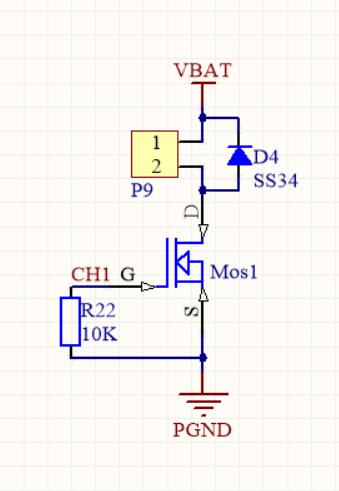
\includegraphics[scale=0.4]{mos.jpg}
	\caption{有刷电机驱动电路}
	\label{fig:label}
\end{figure}

我们可以通过控制在一个周期内,mos管导通的时间,来等效地控制电压。这就是常见的PWM控制。只要PWM的频率高到一定程度,控制效果就接近于直接改变电压来控制速度。(一般使用8K-25K的频率)至于为什么不用三极管而用Mos管,主要原因是:三极管管压降(Vce)大,会有较大电压浪费在三极管上。

图中的R22是一个下拉电阻,保证在单片机刚上电时引脚悬空的时候,mos不会误触发成导通状态。D4是续流二极管,在Mos关闭状态,给电机的电流一个续流通道,否则mos管D极的感应电动势可能会击穿mos。

单片机输出PWM波的引脚必须是定时器(如TIM1),因此分配引脚的时候要注意不要分配错了。


\subsection{舵机控制电路设计}
前面提到,控制舵机是使用PWM信号,因此直接从单片机引出一个能输出PWM波的引脚,与另外两个插针(3.7V,GND)组成了舵机的接口。

需要注意的是,控制舵机的电流不是由单片机产生的,不要想当然的认为是单片机的高电平驱动了舵机。单片机只提供了一个信号给舵机自己的控制电路。

\subsection{通信电路设计}
通信部分我们使用一个蓝牙串口,较为简单。实际上更为常用的是使用NRF24L01等无线射频芯片来达到较为远距离的传输。但出于设计简单考虑,我们还是选择蓝牙。

蓝牙的电路参考说明手册进行连接即可,需要注意的是,蓝牙的RX需接单片机串口的TX,蓝牙的TX需接单片机的RX,接反会无法接受数据。(普通的串口接法)

\subsection{电源部分设计}
单片机及传感器一般使用的电压为3.3V,因此我们需要一个3.7V降为3.3V的电路。一般使用LDO(线性稳压器,与之相对的是开关稳压器,感兴趣的同学可以去查查)。

处于体积考虑,我们选择了sot23-6封装的RT9193,引脚连接参考官方手册。

\begin{figure}[ht]
	\centering
	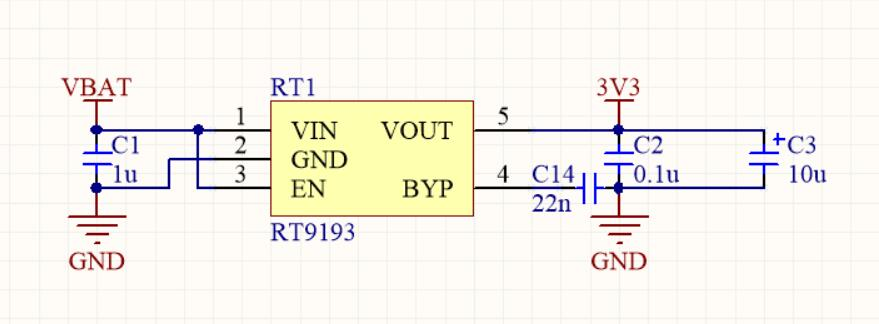
\includegraphics[scale=0.4]{rt9193.jpg}
	\caption{电源电路}
	\label{fig:label}
\end{figure}

\subsection{其他电路设计}
出于拓展考虑,我还在电路板上设计了一个MPU9250及其相应电路。MPU9250是一个9轴传感器,可测三轴角速度、三轴加速度、三轴磁场强度。可以通过对这些信息进行解算,得出俯仰角、横滚叫、偏航角,并实现自动控制。

当然,这是比较高的要求了,没有基础的同学可以略过。

\section{绘制电路板}
绘制电路板的教程这里就不写了,参考视频教程。
需要注意的是,视频中对过孔大小的描述为10mil 10mil是错误的,一般PCB厂的加工能力为12mil,20mil,因此打过孔的时候,尽量打成12mil,20mil。如果过孔孔径超出PCB厂加工能力,工程师会帮你自动调整,但如果板子面积较小无法自动调整,可能会打回修改。因此过孔大小尽量设置为12mil,20mil。


\section{编写控制程序}
\subsection{STM32QubeMX简介}
\subsection{要实现的功能概览}
作为一个飞行器,首先肯定要能驱动飞行器上的电机、舵机等,同时要能接受远程控制的信息,对遥控指令进行响应。

概括一下:
电机、舵机驱动(需要相应定时器引脚,电机与舵机的驱动频率不同,因此必须为不同的定时器)

蓝牙遥控(需要一个USART串口)

\subsection{使用STM32QubeMX帮我们配置初始工程}
新建工程,搜索我们要的芯片型号:STM32F103C8T等,可以仅输入到F103,具体的型号可以再选择。
\begin{figure}[ht]
	\centering
	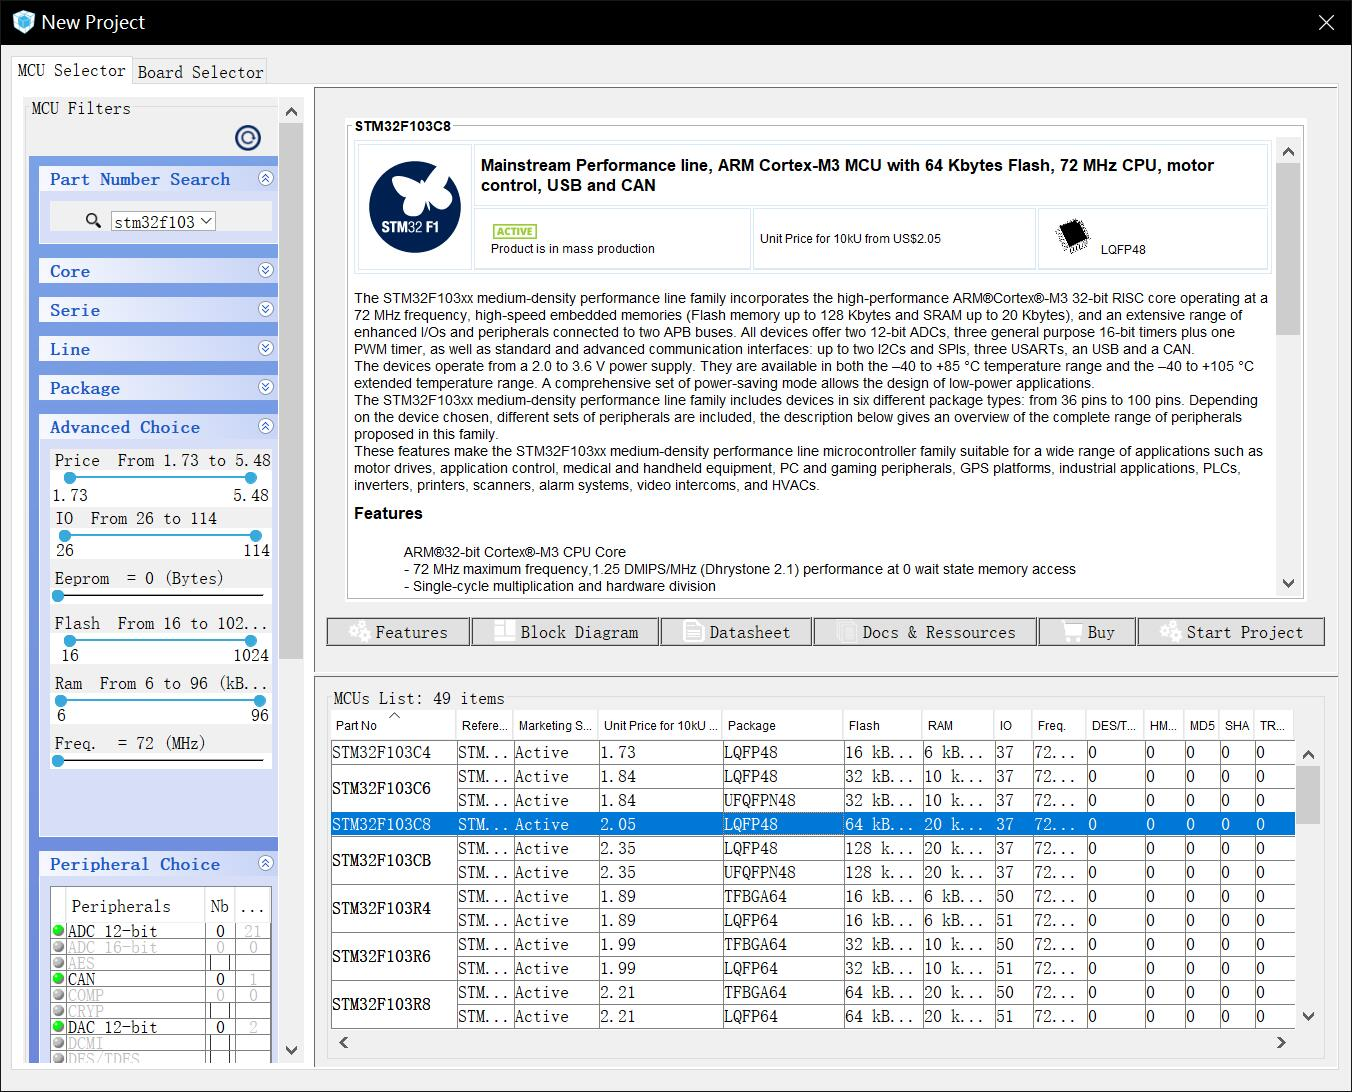
\includegraphics[scale=0.3]{Qube界面.jpg}
	\caption{STM32QubeMX芯片选择界面}
	\label{fig:label}
\end{figure}

首先,配置晶振。晶振产生的时钟信号是整个单片机的时钟来源(虽然很多单片机都有内部振荡器,当没有外部晶振时可以作为替代,但精度等都比不上外部晶振)。

点击Pin\_Out-RCC-High Speed Clock中,选择crystal,即表示我们使用外部晶振。
在Clock Configuration 中,输入Input frequence 为8M,并在HCLK中输入72M,然后按回车,软件会自动帮我们选择合适的倍频系数等等。

\begin{figure}[ht]
	\centering
	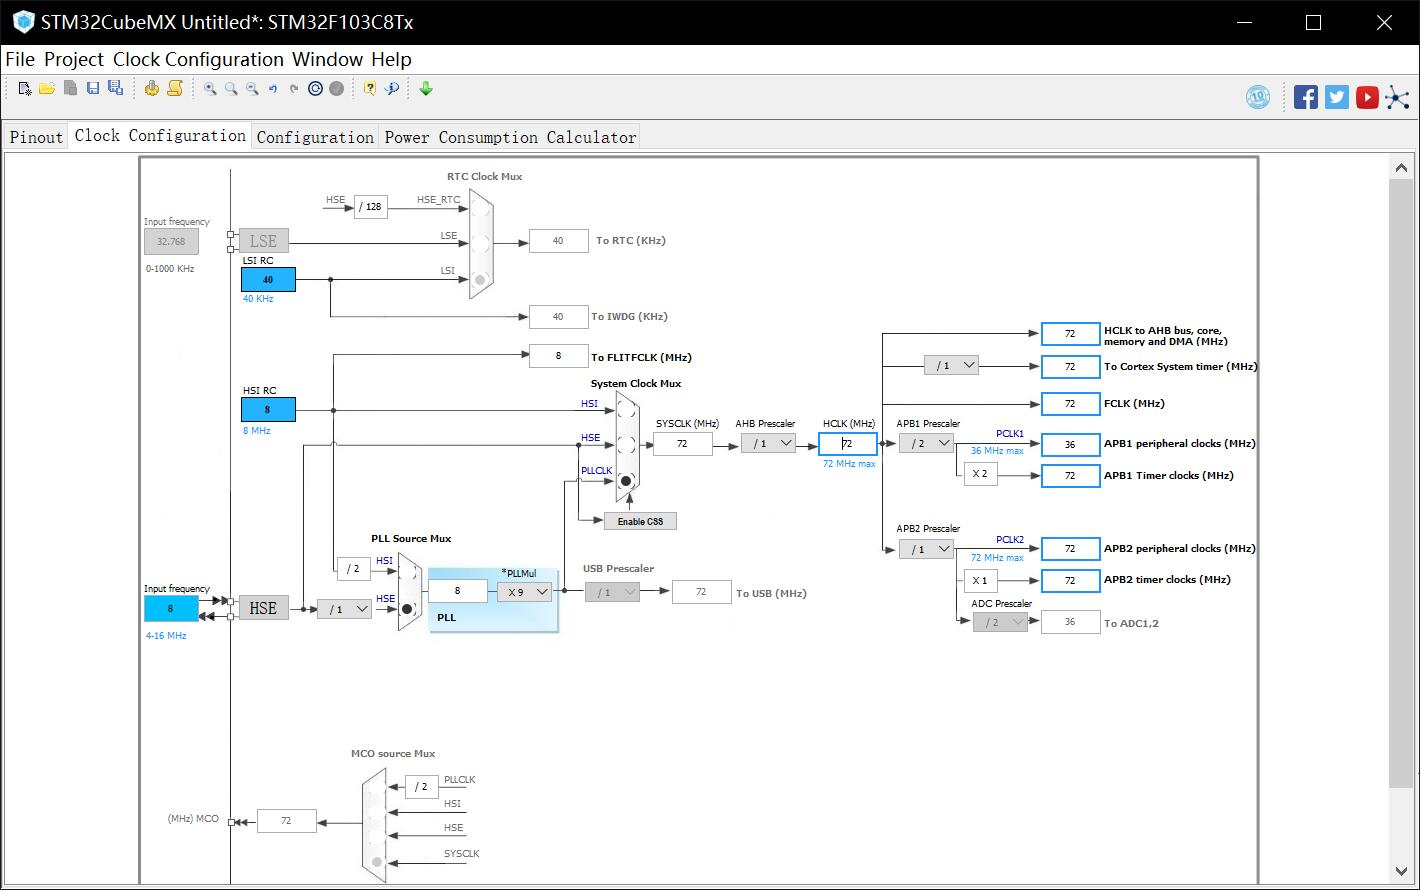
\includegraphics[scale=0.3]{时钟配置.jpg}
	\caption{时钟配置}
	\label{fig:label}
\end{figure}

接下来配置我们要使用的引脚,需要注意的是,有些引脚是不能用的(或者说用了之后会非常麻烦),比如说晶振引脚、下载引脚、调试引脚等,这些引脚最好不要使用。

我们要输出两种频率的PWM波,显然需要两个定时器。至于选用哪个定时器,如果没有特殊情况,应该是在PCB设计时候就决定了(即用哪个定时器好走线)。

因此,我们决定使用TIM4作为空心杯电机的驱动信号(频率8K),TIM1作为舵机的驱动信号(频率50)。由于有两个空心杯电机和两个舵机,每个定时器都使用两个通道(Channel)

配置定时器,在Pin\_Out中,选择TIMn,然后选择我们要使用的通道,选择PWM generation Chn。
这里只是配置了定时器的引脚,关于定时器的频率、PWM占空比等设置,在Configuration中,Control分栏下面,会有各个定时器。双击定时器,即出现参数设置。
我们要设置的参数仅有几个,Prescaler(预分频系数)、Counter\_Period(自动装载值,字面上理解是定时器周期),以及每个通道的Pulse。
其中,预分频系数与自动装载值决定了该定时器所有通道PWM的频率,每个通道的Pulse决定了该通道的占空比。

频率计算公式为:
\begin{equation}
f_o=F/((pre+1) * count\_period)
\end{equation}
F为定时器信号源频率,如果前面按照我说的那样配置时钟的话,那么F=72M。因此,如果我们要使频率为50HZ,参数可取:pre=71,count\_period=20000
频率为8K的参数请大家自行计算。

占空比计算公式为:
\begin{equation}
duty=pulse/count\_priod*100\%
\end{equation}

因为我们是通过改变占空比来实现调速的,因此实际上这个Pulse初值可以不用管,设为0就行了。

接下来配置串口。
点击Pin\_Out ,选择PCB设计已经选好的串口,如USART2,模式选择异步(asynchronous)。
然后设置USART2的参数,默认波特率就是115200,因此不必修改了。


\end{document}